\section{Solution}
\label{sec:solution}

\begin{table*}[!t]
\begin{tabular}{|l|l|l|}
\hline
tweet id & user id & tweet\\
\hline
292375792485298176&858488612& \#KidCudi - \#EraseMe - The Whizz Bells : http://t.co/Lp1zABOV via @youtube\\
292375792481099777&486970282& RT @Kirra\_\_: Today is a day where I need to crawl into my bed and sleep the day away.\\
292375792481099776&336390437& There are poor people, money is the only thing they got.\\
292375792476909568&74570186& I can't do anything without listening to music while I do it.\\
\hline
\end{tabular}
\caption{A sample of the tweet dataset}
\label{tbl:tweets}
\end{table*}


We describe here the PACT program diagram we implemented to produce the statistics on tweets that we want. 
To recap briefly, a PACT program is a generalization of the Map-Reduce paradigm, in which sequence of second order functions are issued in parallel and combined to execute complex tasks. 
The PACT programming paradigm defines 5 second order functions: map, reduce, match, cross and co-group.
It allows the user to specify any kind of combination between them, in any order.
We propose a flow that uses all the operator except the cross. 
For ease of explanation we describe the PACT program as composed in two different blocks: data cleaning (Section~\ref{sec:cleaning}) and the computation of the statistics (Section~\ref{sec:statistics}).

\subsection{Data cleaning}
\label{sec:cleaning}
In the data cleaning part we take in input a comma separated file having the format $\langle tweet\_id$,$user\_id$,$tweet \rangle$. 
Table~\ref{tbl:tweets} shows an excerpt of the tweet tuples. 
Note that it is not always easy to find interesting information from arbitrarily short-texts.
Therefore, we propose a first flow that removes useless or uniformative tweets. 
Figure~\ref{fig:cleaning} depicts the sequence of operations we designed to clean the data in the preliminary phase. 

Once we loaded the tweets into tuples we clean them, from hashtags, user-mentions and urls. 
Tweets are then used in two separate flows: (1) we split them into words in order to count the english words and (2) we perform a sentiment analysis over the text, in order to polarize them into positive and negative, as described in~\ref{sec:introduction}.

In order to restrict the search space to those tweets we consider relevant, we import a dictionary of english words and we count english words in each tweet. 
If a tweet has a percentage of english words greater than a threshold $\sigma$ we keep it, otherwise we drop it. 

From the pruned tweets we extract the users and we match the polarities found in the previous steps. 

\begin{figure*}[ht]
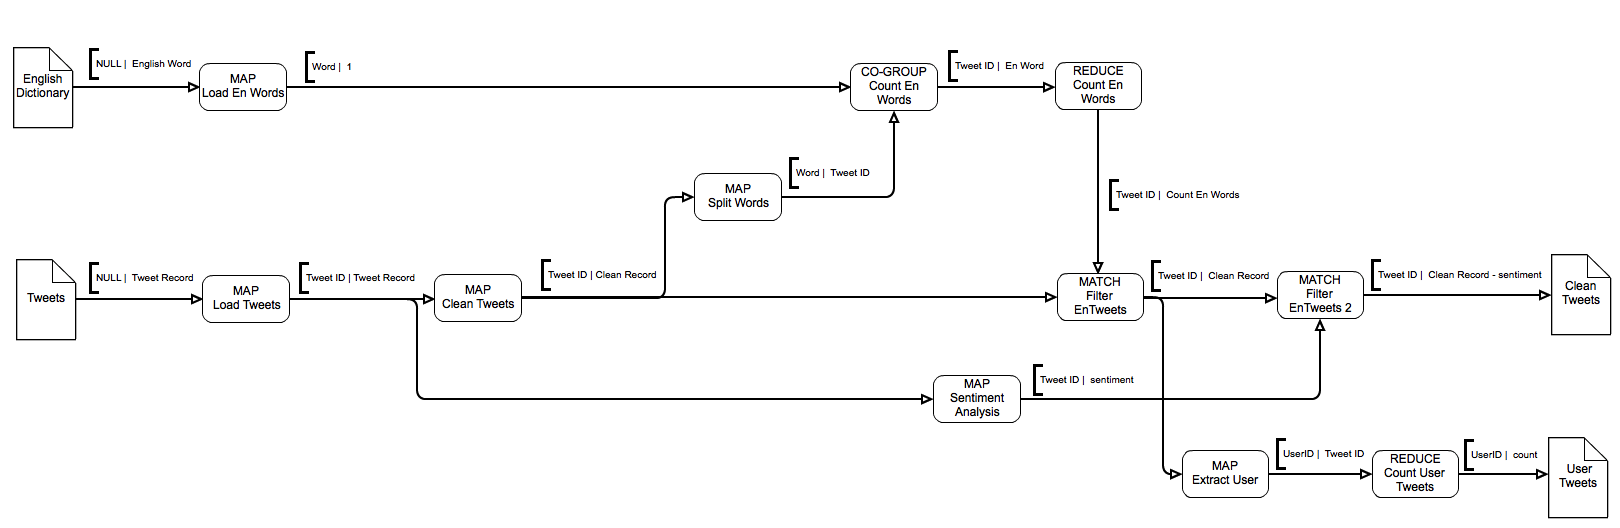
\includegraphics[width=\textwidth]{images/strato_pact_pt1.png} 
\caption{Data cleaning PACT}
\label{fig:cleaning}
\end{figure*}

\subsection{Compute statistics}
\label{sec:statistics}
After having cleaned the raw data we compute the statistics using the tuples we have kept in the previous steps. 
First, we load and match the tuples with the tweet timestamp we get from the database. 
Second, we compute match the hashtags with the polarities in order to understand positive and negative trends of the topics. 
This step is performed by a match operation with the sentiment polarities followd by a sequence of reduce to sum the polarities per tweet, per hashtag and {\bf MATTEO - This part is better described by you}.

\begin{figure*}[ht]
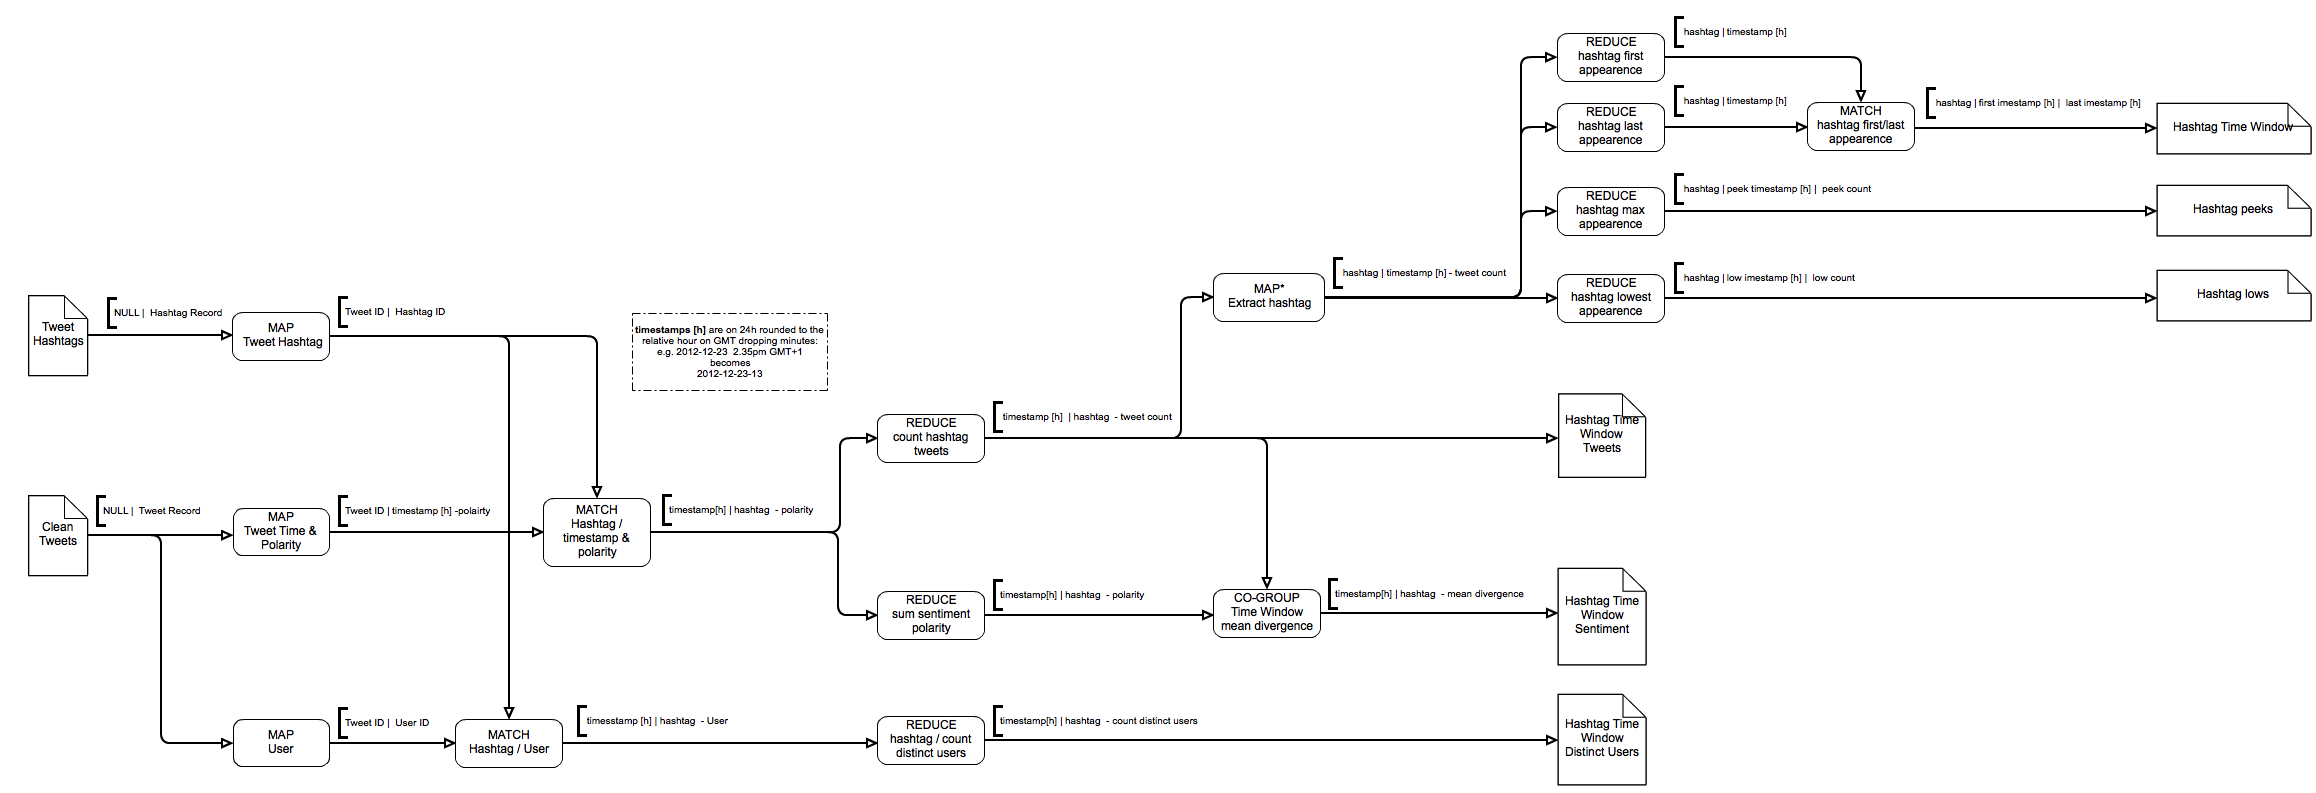
\includegraphics[width=\textwidth]{images/strato_pact_pt2.png} 
\caption{Compute statistics PACT}
\label{fig:statistics}
\end{figure*}
